\chapter{Motivación}

A continuación se dan a conocer algunas de las posibles aplicaciones de un electromiógrafo. \\

\section{Programa de microswitches}

Personas con severas y múltiples discapacidades usualmente son incapaces de interactuar con el entorno que los rodea o reaccionar ante estímulos relevantes debido a su limitado repertorio motor, una posible manera de ayudarlos a superar este tipo de problemas es por medio de la implementación de programas basados en microswitches \cite{chau2016paediatric}. \\

Para incluir a una persona en este programa se deben satisfacer los siguientes parámetros:

\begin{enumerate}
	\item Identificar una respuesta confiable que pueda ser realizada por la persona y que no implique mucho esfuerzo \cite{chau2016paediatric}.
    \item Un microswitch que monitorice la respuesta y que permita la ocurrencia de la misma al estimular algun objetivo \cite{chau2016paediatric}.
    \item Un objetivo de estimulación que la persona encuentre relevante para activar \cite{chau2016paediatric}.
\end{enumerate}


\begin{figure}[h]
  \centering
  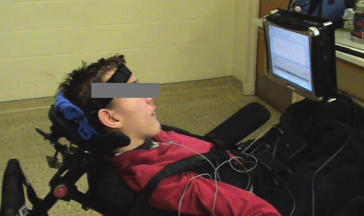
\includegraphics[width=0.5\textwidth]{Contexto/microswitch.jpg}
  \caption{Programa de microwitches \cite{chau2016paediatric}}
  \label{microswitch} 
\end{figure}

John sufre parálisis cerebral cuadripléjica distónica, sus métodos de comunicación consisten e sistemas de comunicacion y exploracion asistida, o instrumentos de habla limitada \cite{chau2016paediatric}. \\

La única frase que puede articular es "ya" y debido a la lejanía del micrófono y a los movimientos bruscos e involuntarios de brazos y cabeza, el instrumento de habla limitada era susceptible a percibir ruidos, de igual modo el uso de switches infrarrojos en sus manos presentaba un problemas por los movimientos continuos \cite{chau2016paediatric}. \\

El único movimiento que podía ejecutar repetidamente y sin mucho esfuerzo consistía en levantar las cejas por ende se opto por un sensor MMG (Mecanomiógrafo) para monitorizar esta señal de control \cite{chau2016paediatric}, Figura \ref{John}. \\

Jane sufre parálisis cerebral cuadriplejica distópica, hace uso de un interruptor en su cabeza y una interfaz dynavox para comunicarse, el switch en su cabeza debía ser reposicionado continuamente debido a los espasmos que sufría, no obstante podía llevar a cabo movimientos voluntarios del pulgar, en un inicio se planeo usar un sensor infrarrojo o de flexión pero debido a la magnitud de los movimientos se opto por MMG \cite{chau2016paediatric}, Figura \ref{Jane}. \\

Ahora bien es conveniente hacer una serie de aclaraciones con respecto a los mecanomiógrafos:

\begin{enumerate}
	\item Un MMG se enfoca en las vibraciones de los músculos en vez de su actividad eléctrica.
    \item Es empleado para movimientos musculares de baja intensidad y que a su vez se pueden ver inmersos dentro de un conjunto de movimientos involuntarios.
    \item Las señales tomadas por el sensor fueron limitadas a un rango de frecuencias entre los 5 y los 50 $hz$.
\end{enumerate}

Como se puede entender los principios de operación de un MMG y EMG son algo diferentes, sin embargo la aplicación puede ser la misma en el sentido de que se enfocan en la monitorizacion de la actividad muscular, la idea del proyecto consiste en el desarrollo de un programa de microswitches basado en MMG.

\begin{figure}[H]
\centering
%----------------------------------------------------------
\begin{subfigure}{0.5\textwidth} 
  \centering
  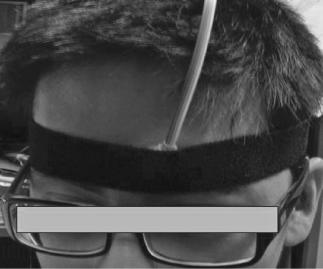
\includegraphics[width=0.5\linewidth]{Contexto/eyebrow.jpg}
  \caption{John}
  \label{John}
\end{subfigure}
%----------------------------------------------------------
\begin{subfigure}{0.5\textwidth}
  \centering
  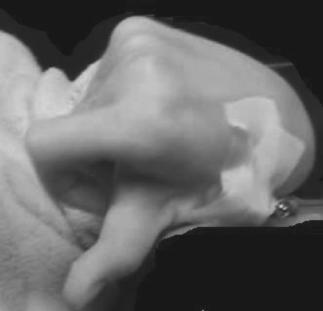
\includegraphics[width=0.5\linewidth]{Contexto/finger.jpg}
  \caption{Jane}
  \label{Jane}
\end{subfigure}
%----------------------------------------------------------
\caption{Usuarios de microswitches \cite{chau2016paediatric}.} 
\label{usos microswitches}
\end{figure}


